\documentclass[12pt,a4paper]{article}
\title{Lab6-Lucene3(自定义Similarity)}
\usepackage{ctex}
\usepackage{amsmath,amscd,amsbsy,amssymb,latexsym,url,bm,amsthm}
\usepackage{epsfig,graphicx,subfigure}
\usepackage{enumitem,balance}
\usepackage{wrapfig}
\usepackage{mathrsfs,euscript}
\usepackage[usenames]{xcolor}
\usepackage{hyperref}
\usepackage[vlined,ruled,commentsnumbered,linesnumbered]{algorithm2e}
\usepackage{float}
\usepackage{geometry}
\usepackage{listings}
\geometry{a4paper,scale=0.8}
\usepackage[T1]{fontenc}
\usepackage[utf8]{inputenc}
\usepackage{amssymb}
% --- Python code template ---
\usepackage[utf8]{inputenc}
% Default fixed font does not support bold face
\DeclareFixedFont{\ttb}{T1}{txtt}{bx}{n}{12} % for bold
\DeclareFixedFont{\ttm}{T1}{txtt}{m}{n}{12}  % for normal

% Custom colors
\usepackage{color}
\definecolor{deepblue}{rgb}{0,0,0.5}
\definecolor{deepred}{rgb}{0.6,0,0}
\definecolor{deepgreen}{rgb}{0,0.5,0}

\usepackage{listings}

% Python style for highlighting
\newcommand\pythonstyle{\lstset{
language=Python,
basicstyle=\ttm,
morekeywords={self},              % Add keywords here
keywordstyle=\ttb\color{deepblue},
emph={MyClass,__init__},          % Custom highlighting
emphstyle=\ttb\color{deepred},    % Custom highlighting style
stringstyle=\color{deepgreen},
frame=tb,                         % Any extra options here
showstringspaces=false
}}
% Python environment
\lstnewenvironment{python}[1][]
{
\pythonstyle
\lstset{#1}
}
{}

% Python for external files
\newcommand\pythonexternal[2][]{{
\pythonstyle
\lstinputlisting[#1]{#2}}}

% Python for inline
\newcommand\pythoninline[1]{{\pythonstyle\lstinline!#1!}}

% --- Python code template ---


\title{Lab6\quad Lucene3(自定义Similarity)}
\date{2021.10}
\author{孙济宸\quad \quad 学号:520030910016 \quad  \quad 班级:F2003003}
\begin{document}
\maketitle
\section{实验概览}
\begin{enumerate}
\item 通过重写Lucene的PythonClassicSimilarity函数实现自定义相似度函数,相似度用于创建索引和查找时评分和排序。
\item 通过在爬取的网页中测试,比较重写的相似度函数和lucene默认的相似度函数的差异。
\end{enumerate}
\section{实验环境}
\begin{itemize}
	\item Docker
	\item \textbf{beautifulsoup (bs4)}
	\item \textbf{pylucene}
	\item \textbf{jieba}
	\item \textbf{paddle}: jieba启用paddle功能依赖库;需运行pip install paddlepaddle

\end{itemize}
\newpage

\section{练习题的解决思路}
通过重写PythonClassicSimilarity类,得到2个自定义相似度类:
其中主要重写了$tf$和$idf$计算方法。
$$tf_1=\sqrt{f_t}, idf_1=\log{\frac{N}{d_f}}$$
$$tf_2=\log{f_t+1}, idf_2=\log{(\frac{N-d_f}{d_f}+1)}$$
\begin{python}
class SimpleSimilarity1(PythonClassicSimilarity):

    def lengthNorm(self, numTerms):
        return 1 / math.sqrt(numTerms)

    def tf(self, freq):
        return math.sqrt(freq)

    def sloppyFreq(self, distance):
        return 1 / (distance + 1)

    def idf(self, docFreq, numDocs):
        return math.log2((numDocs + 1) / (docFreq + 1))

    def idfExplain(self, collectionStats, termStats):
        return Explanation.match(1.0, "inexplicable", [])

class SimpleSimilarity2(PythonClassicSimilarity):

    def lengthNorm(self, numTerms):
        return 1 / math.sqrt(numTerms)

    def tf(self, freq):
        return math.log2(freq + 1)

    def sloppyFreq(self, distance):
        return 1 / (distance + 1)

    def idf(self, docFreq, numDocs):
        return math.log2((numDocs - docFreq) / (docFreq) + 1)

    def idfExplain(self, collectionStats, termStats):
        return Explanation.match(1.0, "inexplicable", [])
\end{python}
在Index和Search代码中分别调用setSimilarity方法即可使用自定义similarity函数。
\begin{python}
SIM = [SimpleSimilarity1(),SimpleSimilarity2()]
- IndexFiles_zhCN_sim.py
config.setSimilarity(SIM[SIM_TYPE])
- SearchFiles_zhCN_sim.py
searcher.setSimilarity(SIM[SIM_TYPE])
\end{python}
\section{代码运行结果}

\subsubsection{“中国美国”}

\begin{figure}[H]
	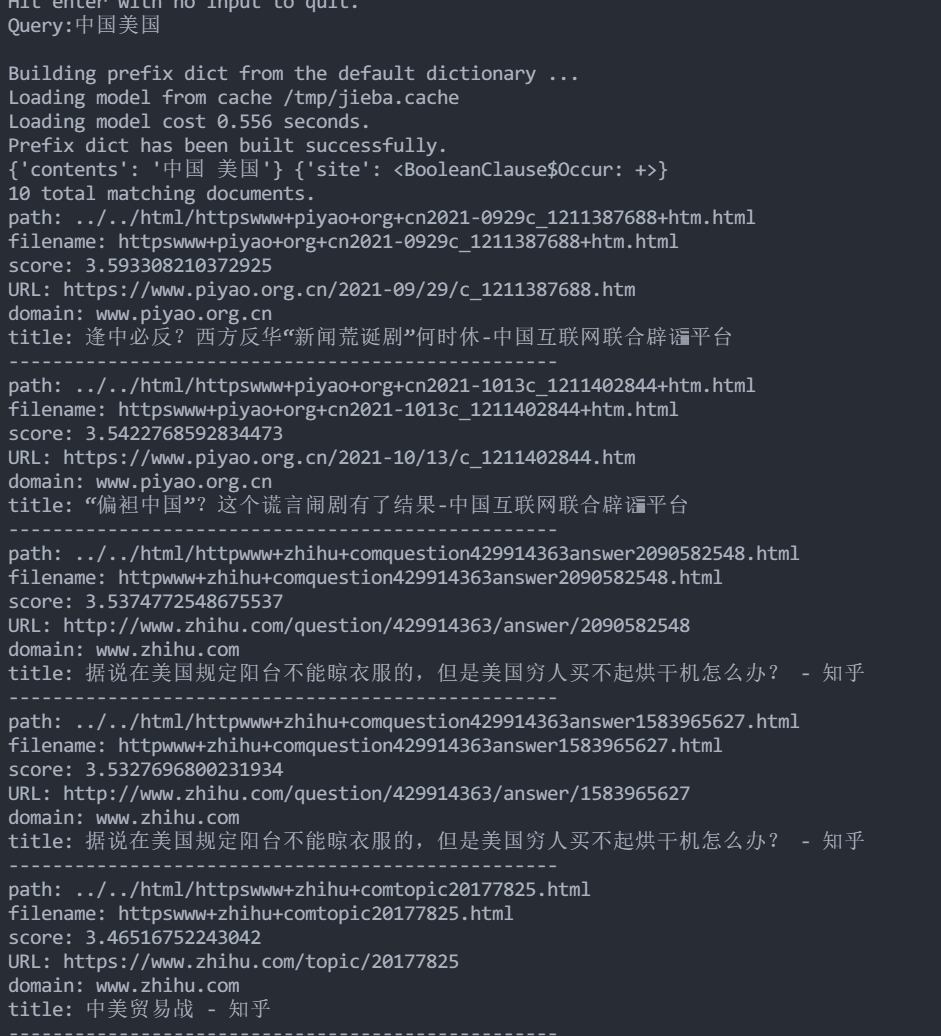
\includegraphics[width=0.6\textwidth]{1_-1.png}
	\centering
	 \caption{默认}
\end{figure}
\begin{figure}[H]
	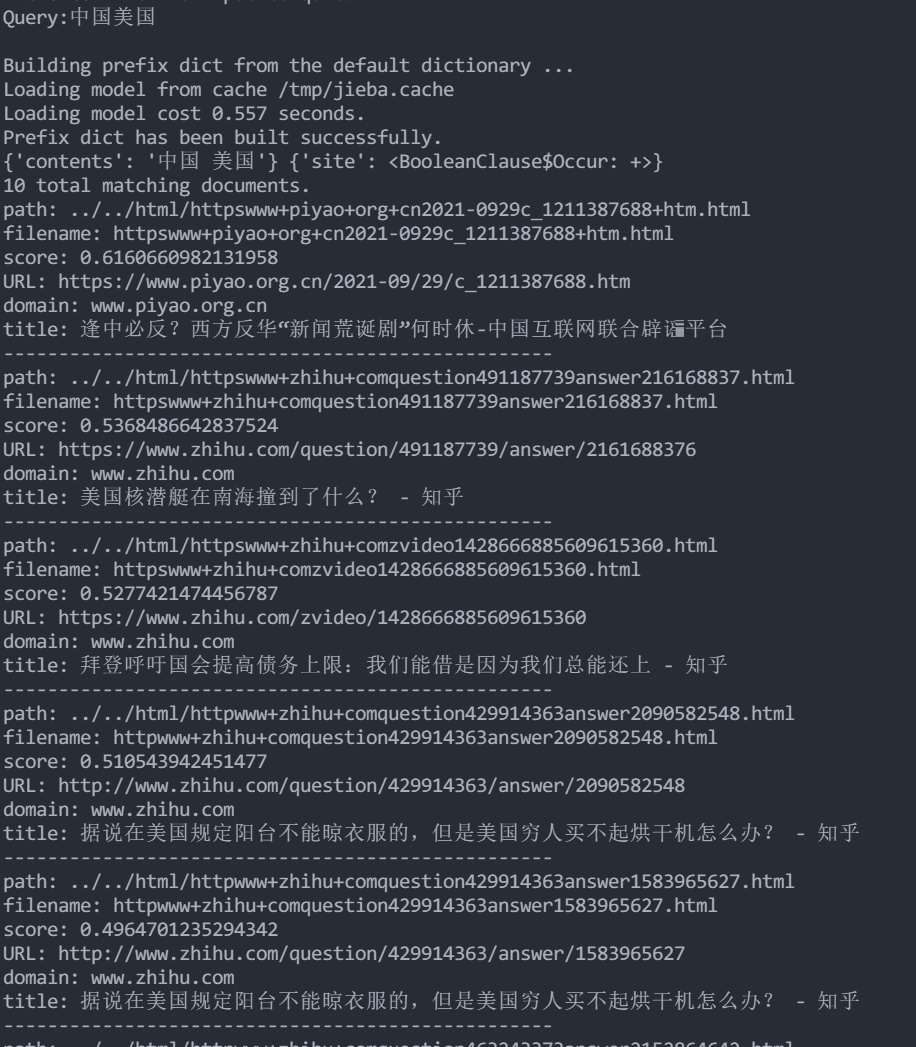
\includegraphics[width=0.6\textwidth]{1_0.png}
	\centering
	 \caption{Similarity0}
\end{figure}
\begin{figure}[H]
	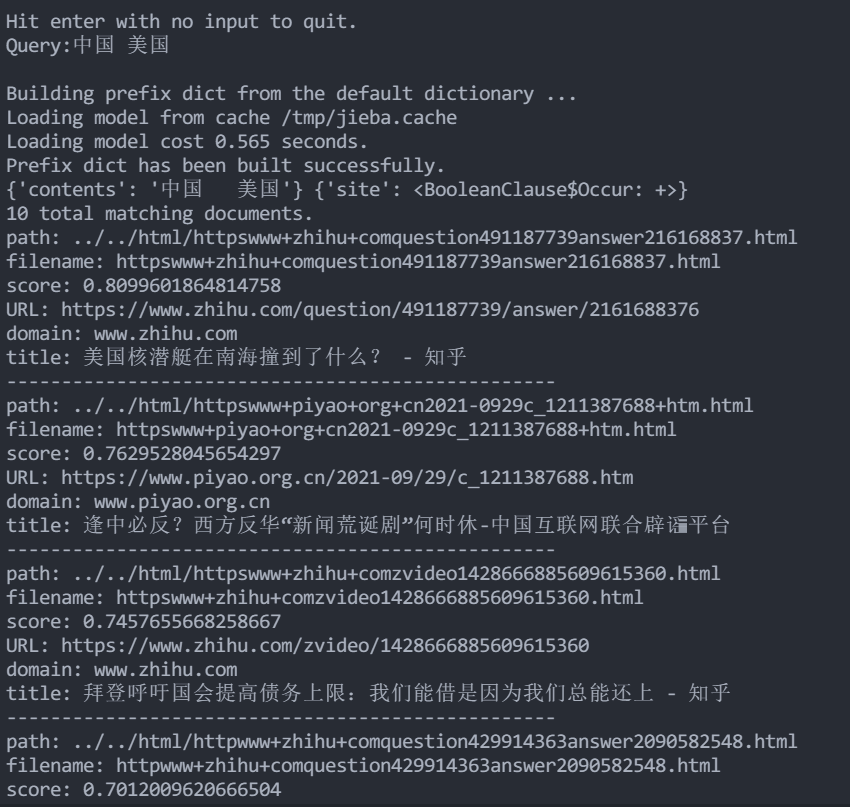
\includegraphics[width=0.6\textwidth]{1_1.png}
	\centering
	 \caption{Similarity1}
\end{figure}

\subsubsection{“最好的编程语言”}

\begin{figure}[H]
	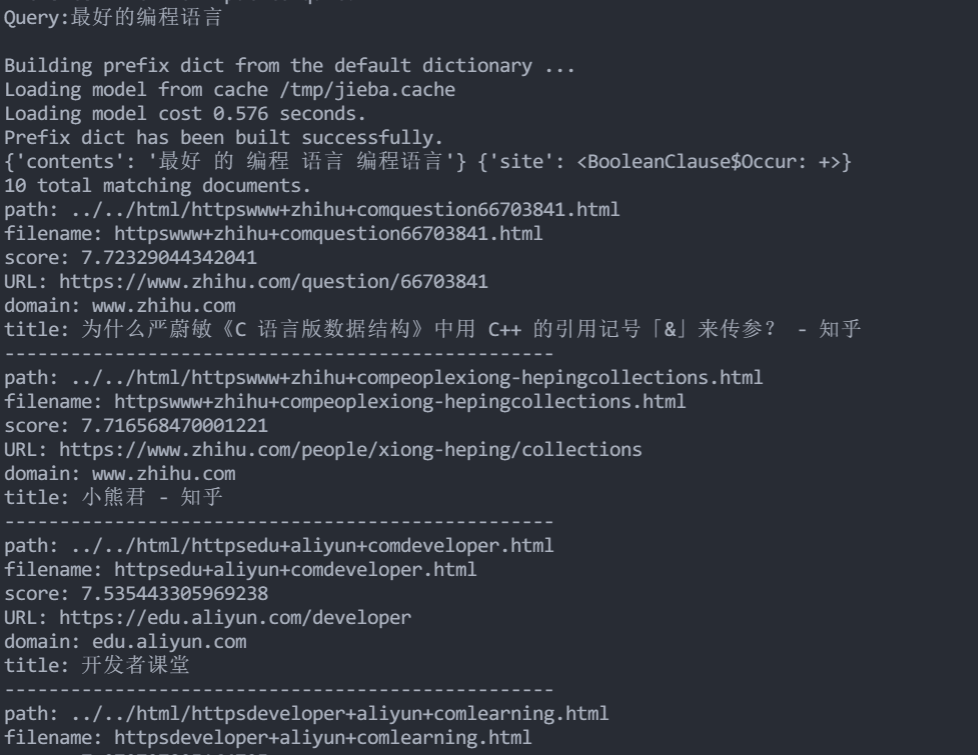
\includegraphics[width=0.6\textwidth]{2_-1.png}
	\centering
	 \caption{默认}
\end{figure}
\begin{figure}[H]
	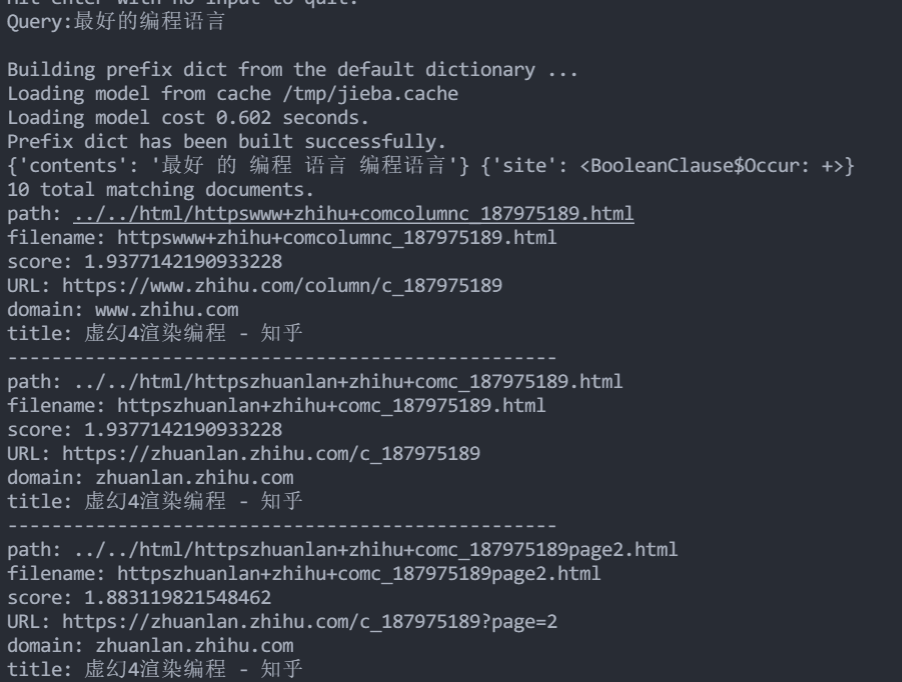
\includegraphics[width=0.6\textwidth]{2_0.png}
	\centering
	 \caption{Similarity0}
\end{figure}
\begin{figure}[H]
	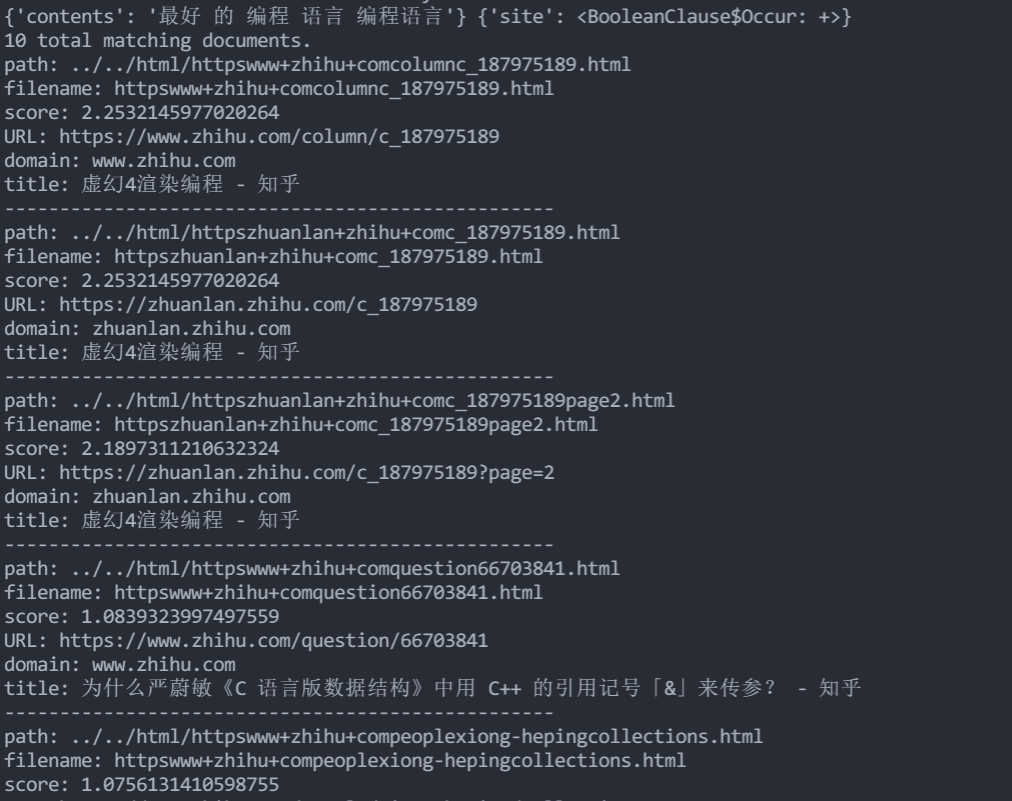
\includegraphics[width=0.6\textwidth]{2_1.png}
	\centering
	 \caption{Similarity1}
\end{figure}

\subsubsection{“中国美食”}

\begin{figure}[H]
	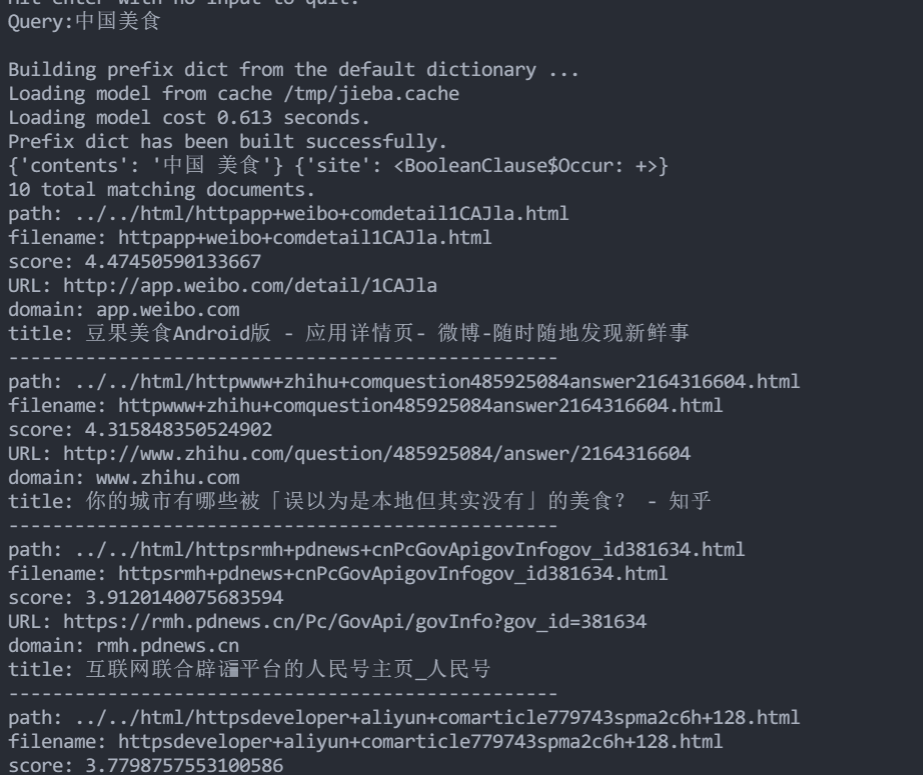
\includegraphics[width=0.6\textwidth]{3_-1.png}
	\centering
	 \caption{默认}
\end{figure}
\begin{figure}[H]
	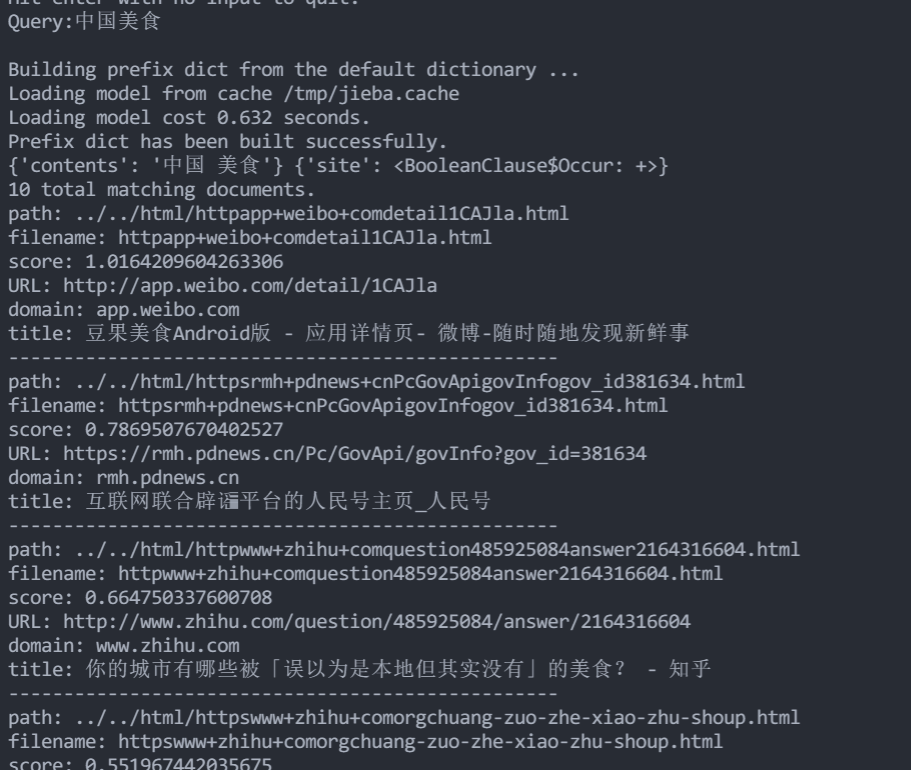
\includegraphics[width=0.6\textwidth]{3_0.png}
	\centering
	 \caption{Similarity0}
\end{figure}
\begin{figure}[H]
	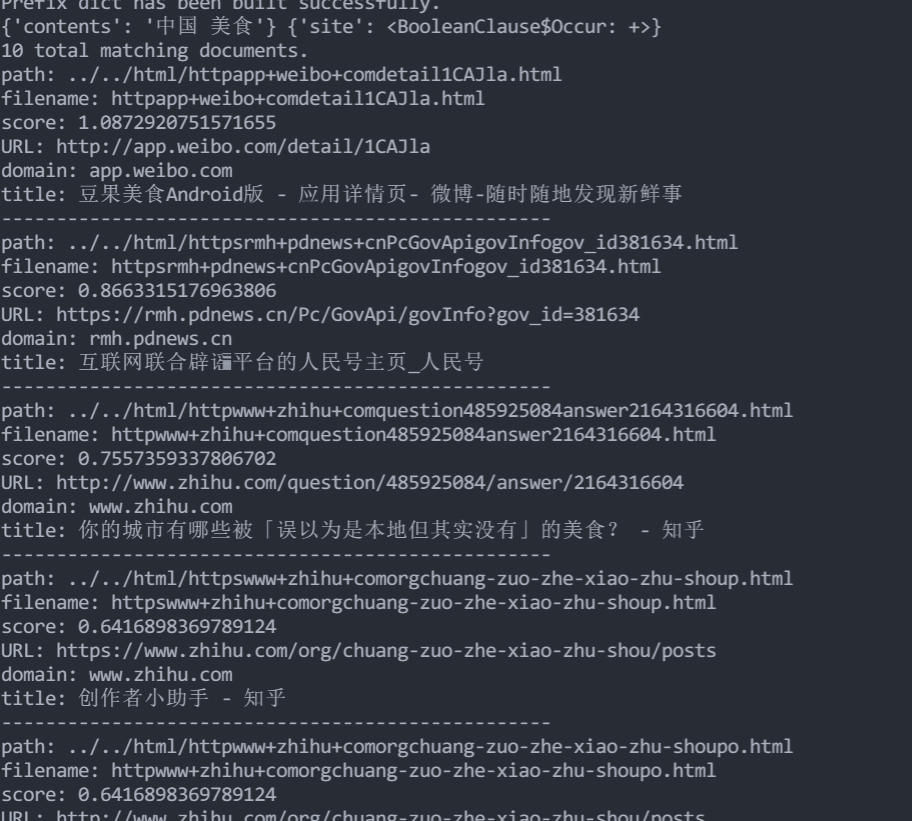
\includegraphics[width=0.6\textwidth]{3_1.png}
	\centering
	 \caption{Similarity1}
\end{figure}

\subsubsection{“搜索引擎”}

\begin{figure}[H]
	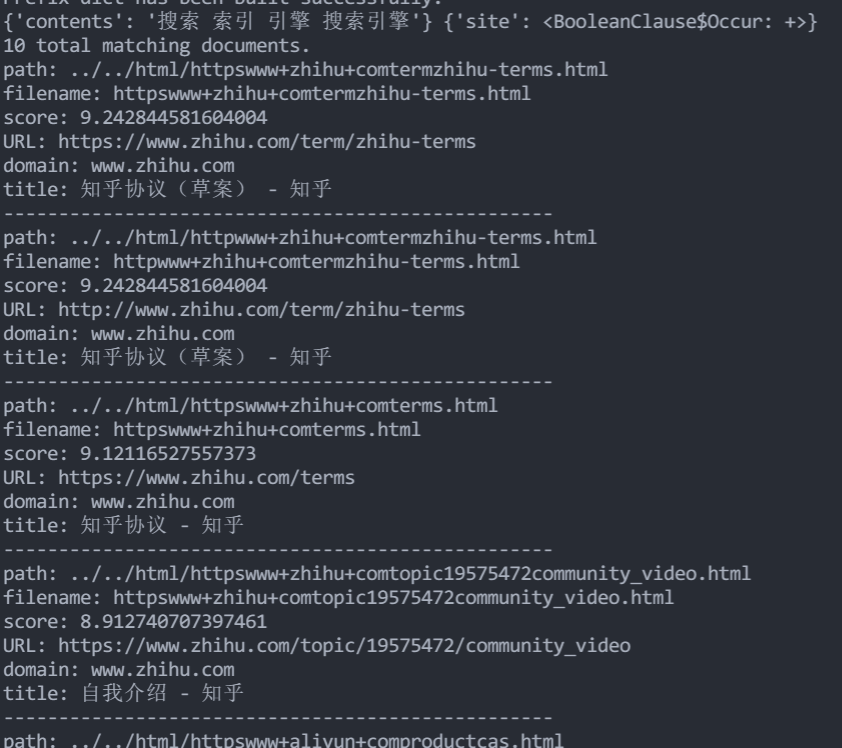
\includegraphics[width=0.6\textwidth]{4_-1.png}
	\centering
	 \caption{默认}
\end{figure}
\begin{figure}[H]
	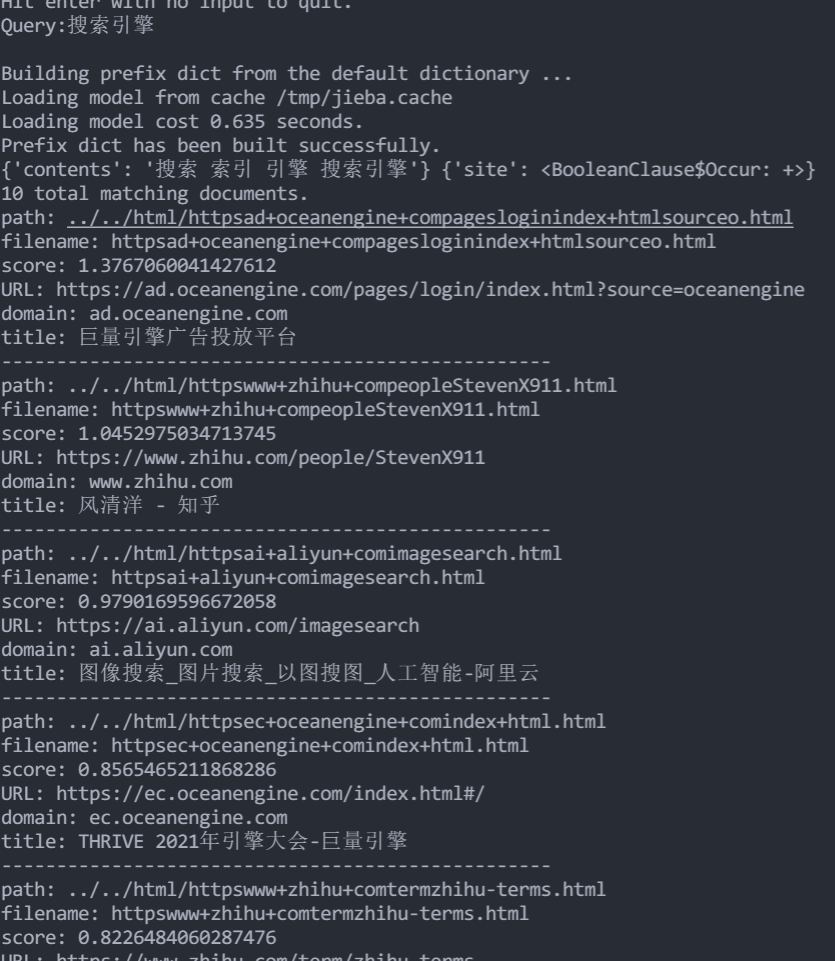
\includegraphics[width=0.6\textwidth]{4_0.png}
	\centering
	 \caption{Similarity0}
\end{figure}
\begin{figure}[H]
	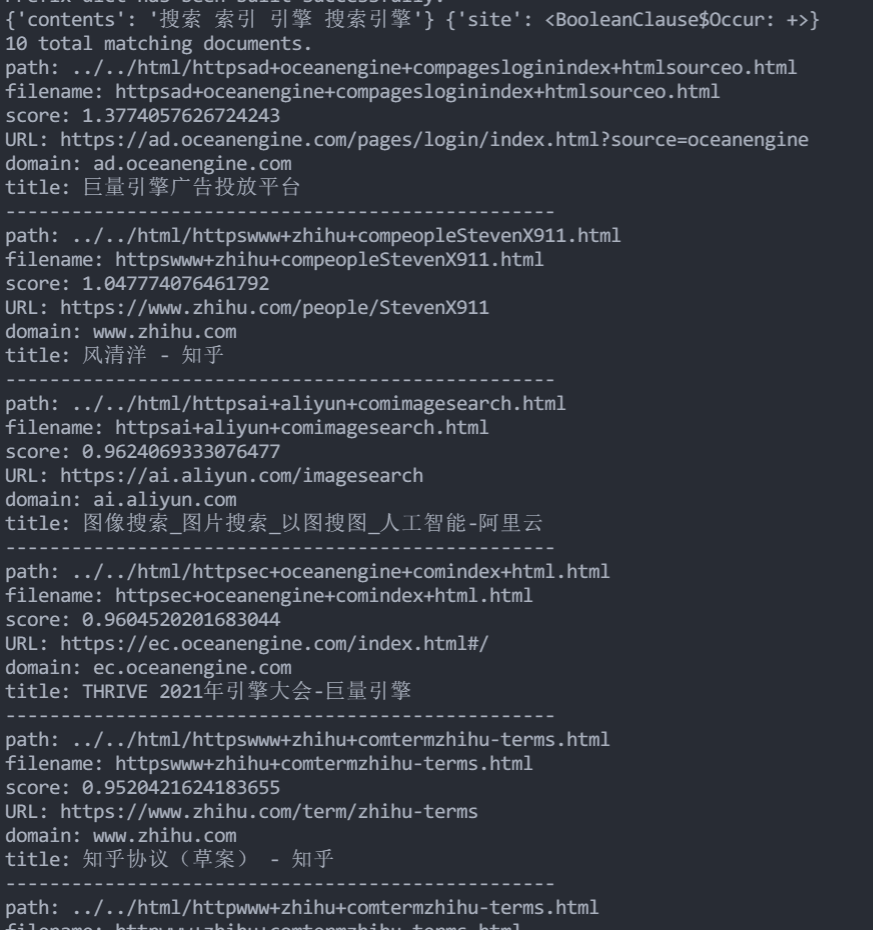
\includegraphics[width=0.6\textwidth]{4_1.png}
	\centering
	 \caption{Similarity1}
\end{figure}

\section{分析与思考}
\begin{itemize}
	\item 从结果来看,用不同函数重写PythonClassicSimilarity对结果影响并不大,但是和Lucene默认方法有一定区别。不同df、idf结果差不多的原因可能是可能是因为测试的网页数目不够大(8000个)或者本身数据对这些变换不敏感。
	\item 观察一些结果可以发现(“搜索引擎”的例子比较明显),重写的tf-idf方法似乎对于keyword出现的次数更敏感,相比之下lucene默认的BM25对全文内容考虑更全面,这二者的优劣有待进一步考量。
\end{itemize}

\end{document}

